
The project was developed using Git as a version control system. All code and issues reported can be found in \href{https://github.com/VolatileSD/ChatServer}{GitHub}. The project is divided in four Main Projects:\\
\begin{itemize}
\item \textbf{ChatServer} - the core of the project: actors, notification API, REST API and database;
\item \textbf{ChatClient} - the GUI Client and Admin;
\item \textbf{NotificationClient} - ZeroMQ based project that allows the client to subscribe the most relevant events in the Chat;
\item \textbf{Common} - utilities and common classes to projects.
\end{itemize}

\subsection{Chat Server}
Most of this project is actor-based. When the server starts, several actors are spawned: two Acceptors, a Room Manager, a Main Room, a Notification Manager and an overall Manager.

\subsubsection{Acceptors.} Each Acceptor is listening on a different port, one for clients that use our text protocol, the other one for the GUI client. This happens mainly because some of the best features are only available in the latter. Every time any of these actors accepts a new connection, an actor \textbf{User} is spawned.

\subsubsection{User.} Each User has an actor named \textbf{LineReader} dedicated to read from his socket. When this actor sends a message (lines it reads from the socket) to the user, it checks if the line starts with the character \textbf{:}. If so, it  checks whether it is a valid command and acts upon that. If not, and when the user is connected to a room, it sends the line to that room.

Every command sends a message to other actors, and most of them need an immediate answer. To achieve this, a special entity, \textbf{Pigeon}, was created. This Pigeon is an important tool in our tool set. It carries a message to any actor and always comes back with an answer.

\subsubsection{Manager.} To better understand this, another essential actor, the \textbf{Manager}, is needed. This actor is in charge of user registration, authentication and removal and private messaging. When the user tries to create an account, this is accomplished with a Pigeon that carries a message to the Manager and retrieves the reply to the User, allowing or preventing the action. After the log in, also achieved with this technique, the user is automatically connected to the Main Room. This room exists by default and it cannot be deleted by any administrator. At this point, the user might try to change to another room. We do this creating another Pigeon but the recipient will be the \textbf{Room Manager}.

\subsubsection{Room Manager.} The Room Manager, besides controlling room changes, is also responsible for room creation and removal. Such requests are made using the \textbf{REST API}, which will be describe further in the document. 
%remove manager from rest aplication
%return false in room when deleting room
When the Room Manager receives a message soliciting a room change, if the rooms exists, it contacts the \textbf{Room} actor, notifying that a user will connect soon. The Room actor counts how many users will connect soon. This will be very important for the REST API. The Room Manager and each Room actor have another important task: send a message to the \textbf{Notification Manager} every time a user enters or leaves a room and every time a room is created or removed.

\subsubsection{Notification Manager.} Every time this actor receives messages, it fowards them to possible connected Notification Clients that subscribed the event that message represents. This is accomplished using 0MQ pub-sub pattern.

\begin{figure}[H]
\centering
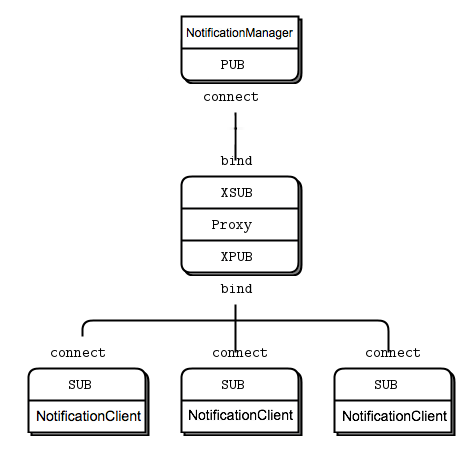
\includegraphics[width=0.6\textwidth]{img/zeromq.png}
\caption{Pub sub}
\label{fig:zmq}
\end{figure}


As we can see in Figure \ref{fig:zmq}, we only have one publisher but we are prepared to add new publishers in the future very easily. The subscribers use our \textbf{Notification API} which we'll discuss further. 

\subsubsection{REST API.}
This project also has a layer that consists in RESTful API using JSON as a serialization format. For detailed information, check the appendix \ref{app:rest}.
The choice of JSON instead of the standard XML results in an increase of performance in terms of serialization and deserialization because JSON is a much more lightweight format. For serialization and deserialization purposes, Gson was mainly used.

When implementing this, we faced a problem. We needed to guarantee that some API calls were only made by admins. For that, this calls request an Header Parameter named \textbf{Volatile-ChatServer-Auth}. This acts as an authentication token. To create this token, we encode a JSON with two properties, username and password, using Base64 encode algorithm. If the username belongs to an admin, and the password is correct, it's a valid token. This mechanism provides no confidentiality protection for the transmitted credentials. They are merely encoded with Base64, but not encrypted or hashed in any way. Therefore, is typically used over HTTPS, which we're not doing. This difficults the use of this calls using a simple client as curl, so we recommend the use of our Chat Client.

There is a situation we took special attention when implementing this API. When a user asks to change room, he will be given the ActorRef to that room. 
Meanwhile, using this API, the admin might try to delete the same room.
The order to delete can arrive before the message from the user notifying his entering, and if so, the user has an ActorRef to a room that will be deleted. This problem was solved with the counter mentioned before: how many users will enter soon. The attempt to delete the room will only succeed if the room has no users and this counter is zero.


\subsubsection{OrientDB} We're using OrientBD \cite{odb} as database. OrientDB is an Open Source NoSQL DBMS with the features of both Document and Graph DBMSs. Our system use it as a Graph Database. Although we do not have a persistence layer, we believe it's a good feature because we can recover the server state if for some reason it crashes.

\subsubsection{Capsule} To deploy our service as a standalone application we use Capsule \cite{capsule}. This allows to package our application into a single JAR and deliver it to anyone who wants to use it. This happens to the Chat Server, Chat Client and Notification Client projects.

\subsection{Chat Client}
\label{subsec:chatclient}
The Chat Client was built for end users. A simple client (e.g. telnet) enjoys almost the same chat features as the GUI client using our text protocol \ref{tab:textprotocol}.
Other features, as listing rooms, choosing a room
and listing users from a room are only accessible using the GUI client. These are calls to our REST API. To also achieve this, the simple client has to use a command line tool like curl or another http client. \\
Another feature is the Inbox. Each client can send private messages to other chat users (even if they are offline) and load their inbox history.

\subsubsection{Text-based protocol}
\label{subsec:textprotocol}
The text-based protocol allows that even simple clients as \textbf{telnet} and \textbf{nc} can enjoy our chat. All protocol components - commands -  start with \textbf{:}. The protocol is as simple as possible so that it would not become too unpleasant for the simple clients.


\begin{table}[h]
\centering
\begin{tabular}{l|l}
\textbf{Command} & \textbf{Description}\\
\hline
\hline
 :h/:help & Lists all available commands \\
 \hline
 :create username password & Creates a new user\\
 \hline
 :remove username passsword & Removes an existing user \\
 \hline
 :login username password & Logs an existing user \\
 \hline 
 :logout & Logs the user out of the service \\
 \hline
 :cr/:changeroom newRoom & Changes the current room to newRoom  \\
 \hline
 :private username message & Sends a private message to a user by username   \\
 \hline
 :inbox & Displays the private messages received
\end{tabular}

\caption{Text protocol for a simple client.}
\label{tab:textprotocol}
\end{table}


\subsubsection{Admin.}
The Admin is a regular chat client with special permissions: it can create new rooms, delete existing ones, promote users to admin and remove their privileges. In the full version, the Admin can easily achieve this because the work of encoding his credentials is done by the application. When using curl he has to use some Base64 encoder for that, which is very distasteful. If the username and password are admin, after encoding the JSON \{"username":"admin", "password":"admin"\} the curl command to create a room is

\small\begin{verbatim}
curl -X PUT -H 
"Volatile-ChatServer-Auth : eyJ1c2VybmFtZSI6ImFkbWluIiwgInBhc3N3b3JkIjoiYWRtaW4ifQ==" 
localhost:8080/room/ROOM
\end{verbatim}


\normalsize



\subsection{Notification Client}
This client uses our Notification API to subscribe relevant events. This API is very similar to REST API endpoints. 

\begin{table}[!h]
\centering
\begin{tabular}{l|l}
\hline
\textbf{:sub rooms} & subscribes rooms creation and removal\\
\hline
\textbf{:unsub rooms} & unsubscribes\\
\hline
\textbf{:sub room/name} & subscribes entries and exists in the room with that name\\
\hline
\textbf{:unsub room/name} & unsubscribes\\
\hline
\end{tabular}
\caption{Notification API}
\end{table}

If in the future our service grows, and we have more publishers notifying other events,
this client demands no change. 

\subsection{Common}
In this project we have the common classes of the whole project. One particular class, Saying, has the replies to all user actions. Each Saying method returns a String, which are used both in Chat Server and Chat Client. It also has representations of important entities that serve as a way to exchange information between the several components.